\appendix

\chapter{Aufgabenstellung}
\label{AnhangAufgabenstellung}

Die Aufgabenstellung wurde im Februar 2018 übergeben und beinhaltet neben der Erläuterung der Aufgabe, weitere Anforderungen und Termine.

Dieses Dokument ist auch im digitalen Angang \ref{AnhangDig} einsehbar.

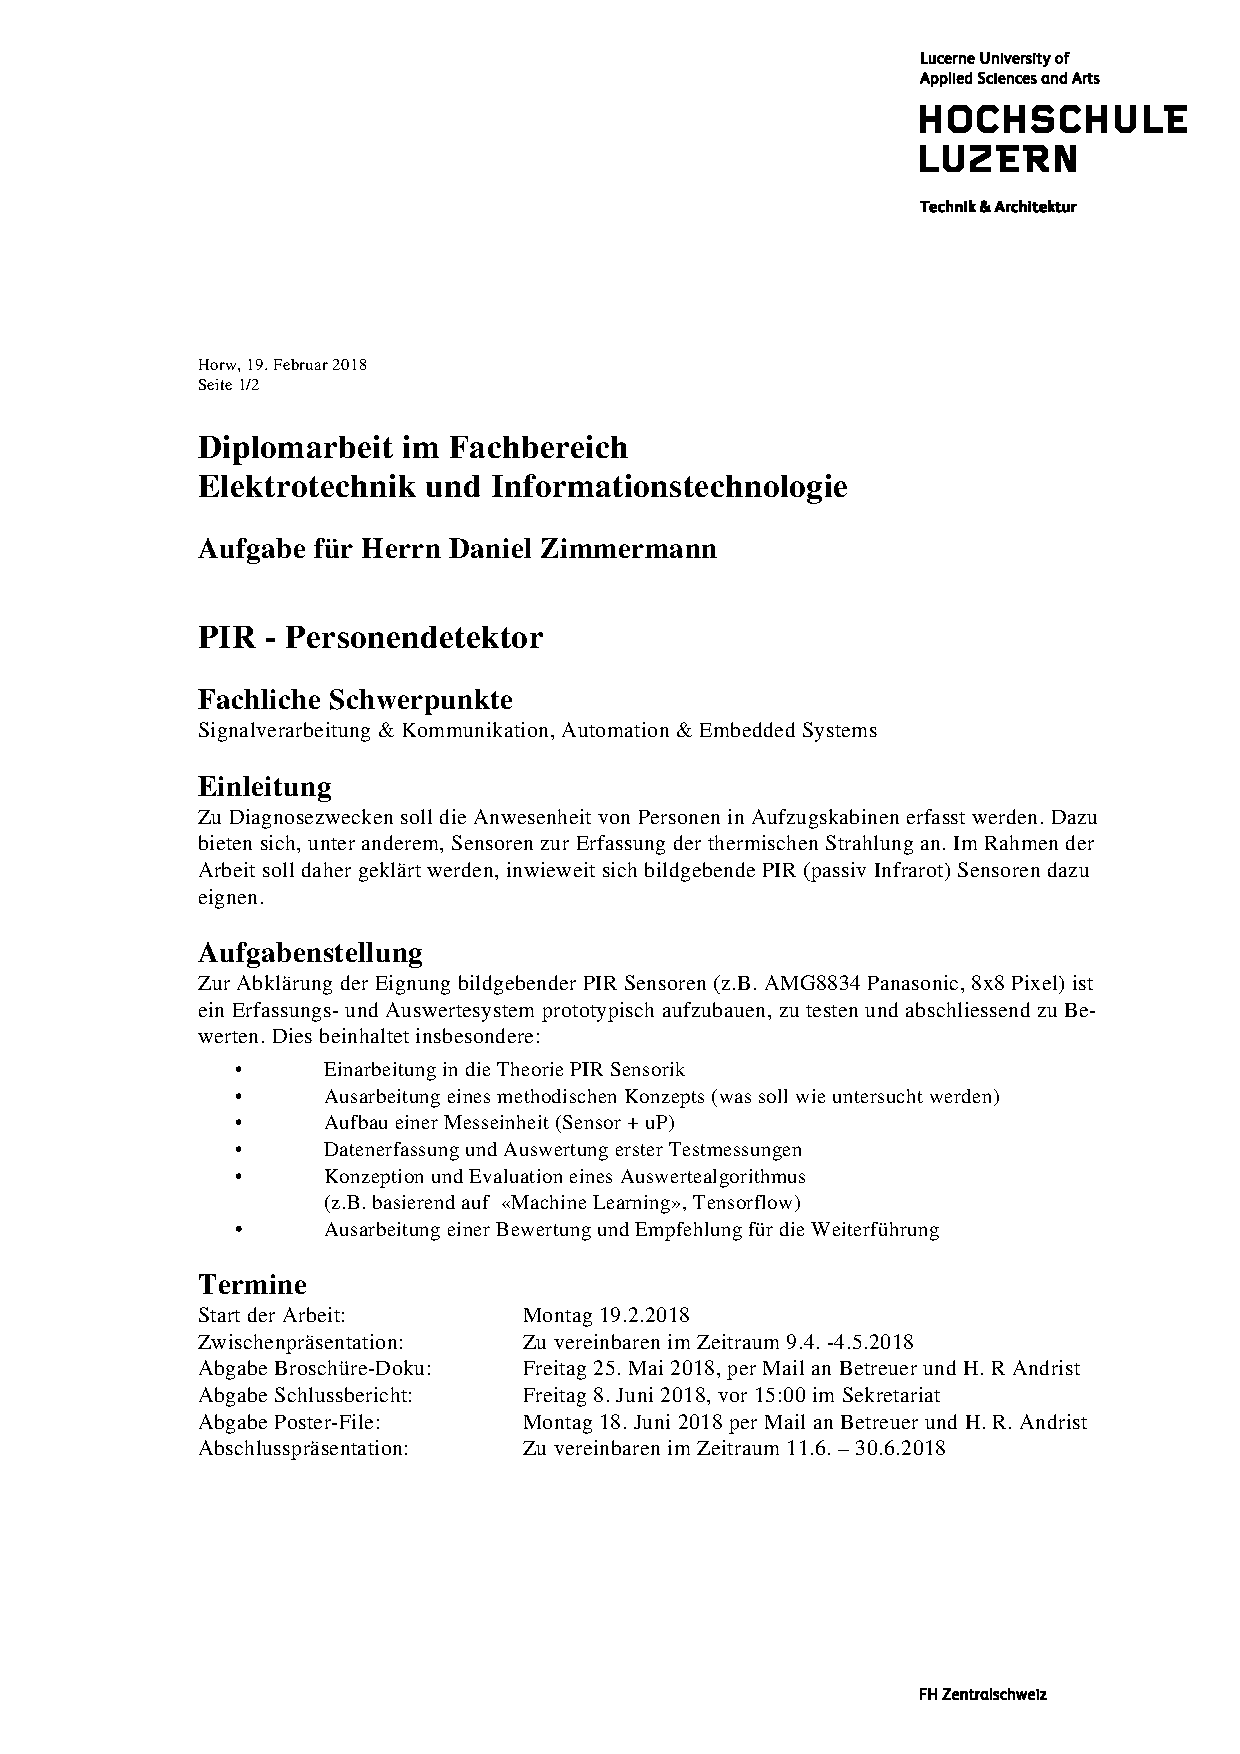
\includepdf[pages=-]{Anhang/Aufgabenstellung.pdf}

\chapter{Meilensteinplan}
Der Meilensteinplan wurde in der Initialisierungsphase erstellt und während dem Projektablauf angepasst. Die Meilensteine wurden farblich unterteilt. Die Unterteilungen sind in der Legende beschrieben. 

Dieses Dokument ist auch im digitalen Angang \ref{AnhangDig} einsehbar.

\label{AnhangA}
\includepdf[pages=1,angle=90]{Anhang/Meilensteinplan_BAT_P1_V3.pdf}

\chapter{Detaillierter Projektplan}
\label{AnhangB}

Der detaillierte Projektplan gibt alle wesentlichen Tätigkeiten während des gesamten Projekt wieder. Dabei sind die Projektabschnitte und die Meilensteine angegeben.

Der Projektplan wurde für eine bessere Übersicht in zwei Teile unterteilt. 
\begin{itemize}
\item Der erste Teil ist der Zeitraum von der Iniitialiiserung bis zur Zwischenpräsentation.

\item Der zweite Teil ist der Zeitruam von der Zwischenpräsentation bis zur Projektbeendigung.

\end{itemize}

Die einzelnen Tätigkeiten wurden auf zeitliche Aufwendungen geschätzt und der effektive Aufwand wird angegeben. 
Jedem Projektabschnitt werden die Zeitaufwendungen separat angerechnet. In jedem Teil ist in \textcolor{yellow}{gelber} Markierung die gesamthafte zeitliche Aufwendung angegeben.


Dieses Dokument ist auch im digitalen Angang \ref{AnhangDig} einsehbar.


%\includepdf[pages=1,angle=90]{Anhang/01_Detaillierter Projektplan BAT V3.pdf}

%\includepdf[pages=1,angle=90]{Anhang/02_Detaillierter Projektplan BAT V3.pdf}



\chapter{Risikomanagement}
\label{AnhangC}
\setcounter{page}{9}
Das Risikomanagement wurde in der Initialisierungsphase erstellt und gibt Auskunft, wleche Risiken bei dieser Arbeit zu beachten sind.

Eine Bewertung der Wahrscheinlichkeit und den Auswirkungen gibt Auskunft, welche Risiken vorrangig beachtet werden müssen.  Dabei wruden die Risiken in Standardrisiken und Projektbezogene Risiken unterteilt.

Dieses Dokument ist auch im digitalen Angang \ref{AnhangDig} einsehbar.

\includepdf[pages=-,angle=90]{Anhang/Risikomanagement_V2.pdf}
\chapter{Übersicht Datensätze }
\label{AnhangD}

Es wird nachfolgend die 3 verschiedene Datensätze aufgezeigt. Dabei werden die wichtisgtsten Eigenschaften der erstellten Profile dargelegt. Neben de Datensätzen werden noch die Eigenschaften des ausgewählten Aufzug. Es werden alle relevatnen Parameter der Aufzugsprofile angegeben. Die erstellten Datensät
